%% ============================================================
%% Chapter 5 — Experimental Setup
%% ============================================================
\chapter{Experimental Setup}
\label{chap:experiments}

\section{Dataset Statistics}
\label{sec:exp_data_stats}

Table~\ref{tab:dataset_stats} summarises the final article-level split.
Figure~\ref{fig:dataset_distribution} provides a visual breakdown. All three
splits are perfectly balanced between answerable and unanswerable questions,
ensuring that a trivial strategy of always answering achieves exactly 50\%
precision when measured on answerability—not 100\%—and that evaluation metrics
are interpretable without correction for class imbalance.

\begin{table}[htbp]
  \centering
  \caption{Dataset split statistics for SQuAD~2.0 (article-level split, seed 42).}
  \label{tab:dataset_stats}
  \begin{tabular}{lrrrr}
    \toprule
    \textbf{Split} & \textbf{Total} & \textbf{Answerable} & \textbf{Unanswerable} & \textbf{Articles} \\
    \midrule
    Train      & 300 & 150 & 150 & 176 \\
    Validation & 100 &  50 &  50 &  61 \\
    Test       & 100 &  50 &  50 &  55 \\
    \midrule
    \textbf{Total} & \textbf{500} & \textbf{250} & \textbf{250} & \textbf{292} \\
    \bottomrule
  \end{tabular}
\end{table}

\begin{figure}[htbp]
  \centering
  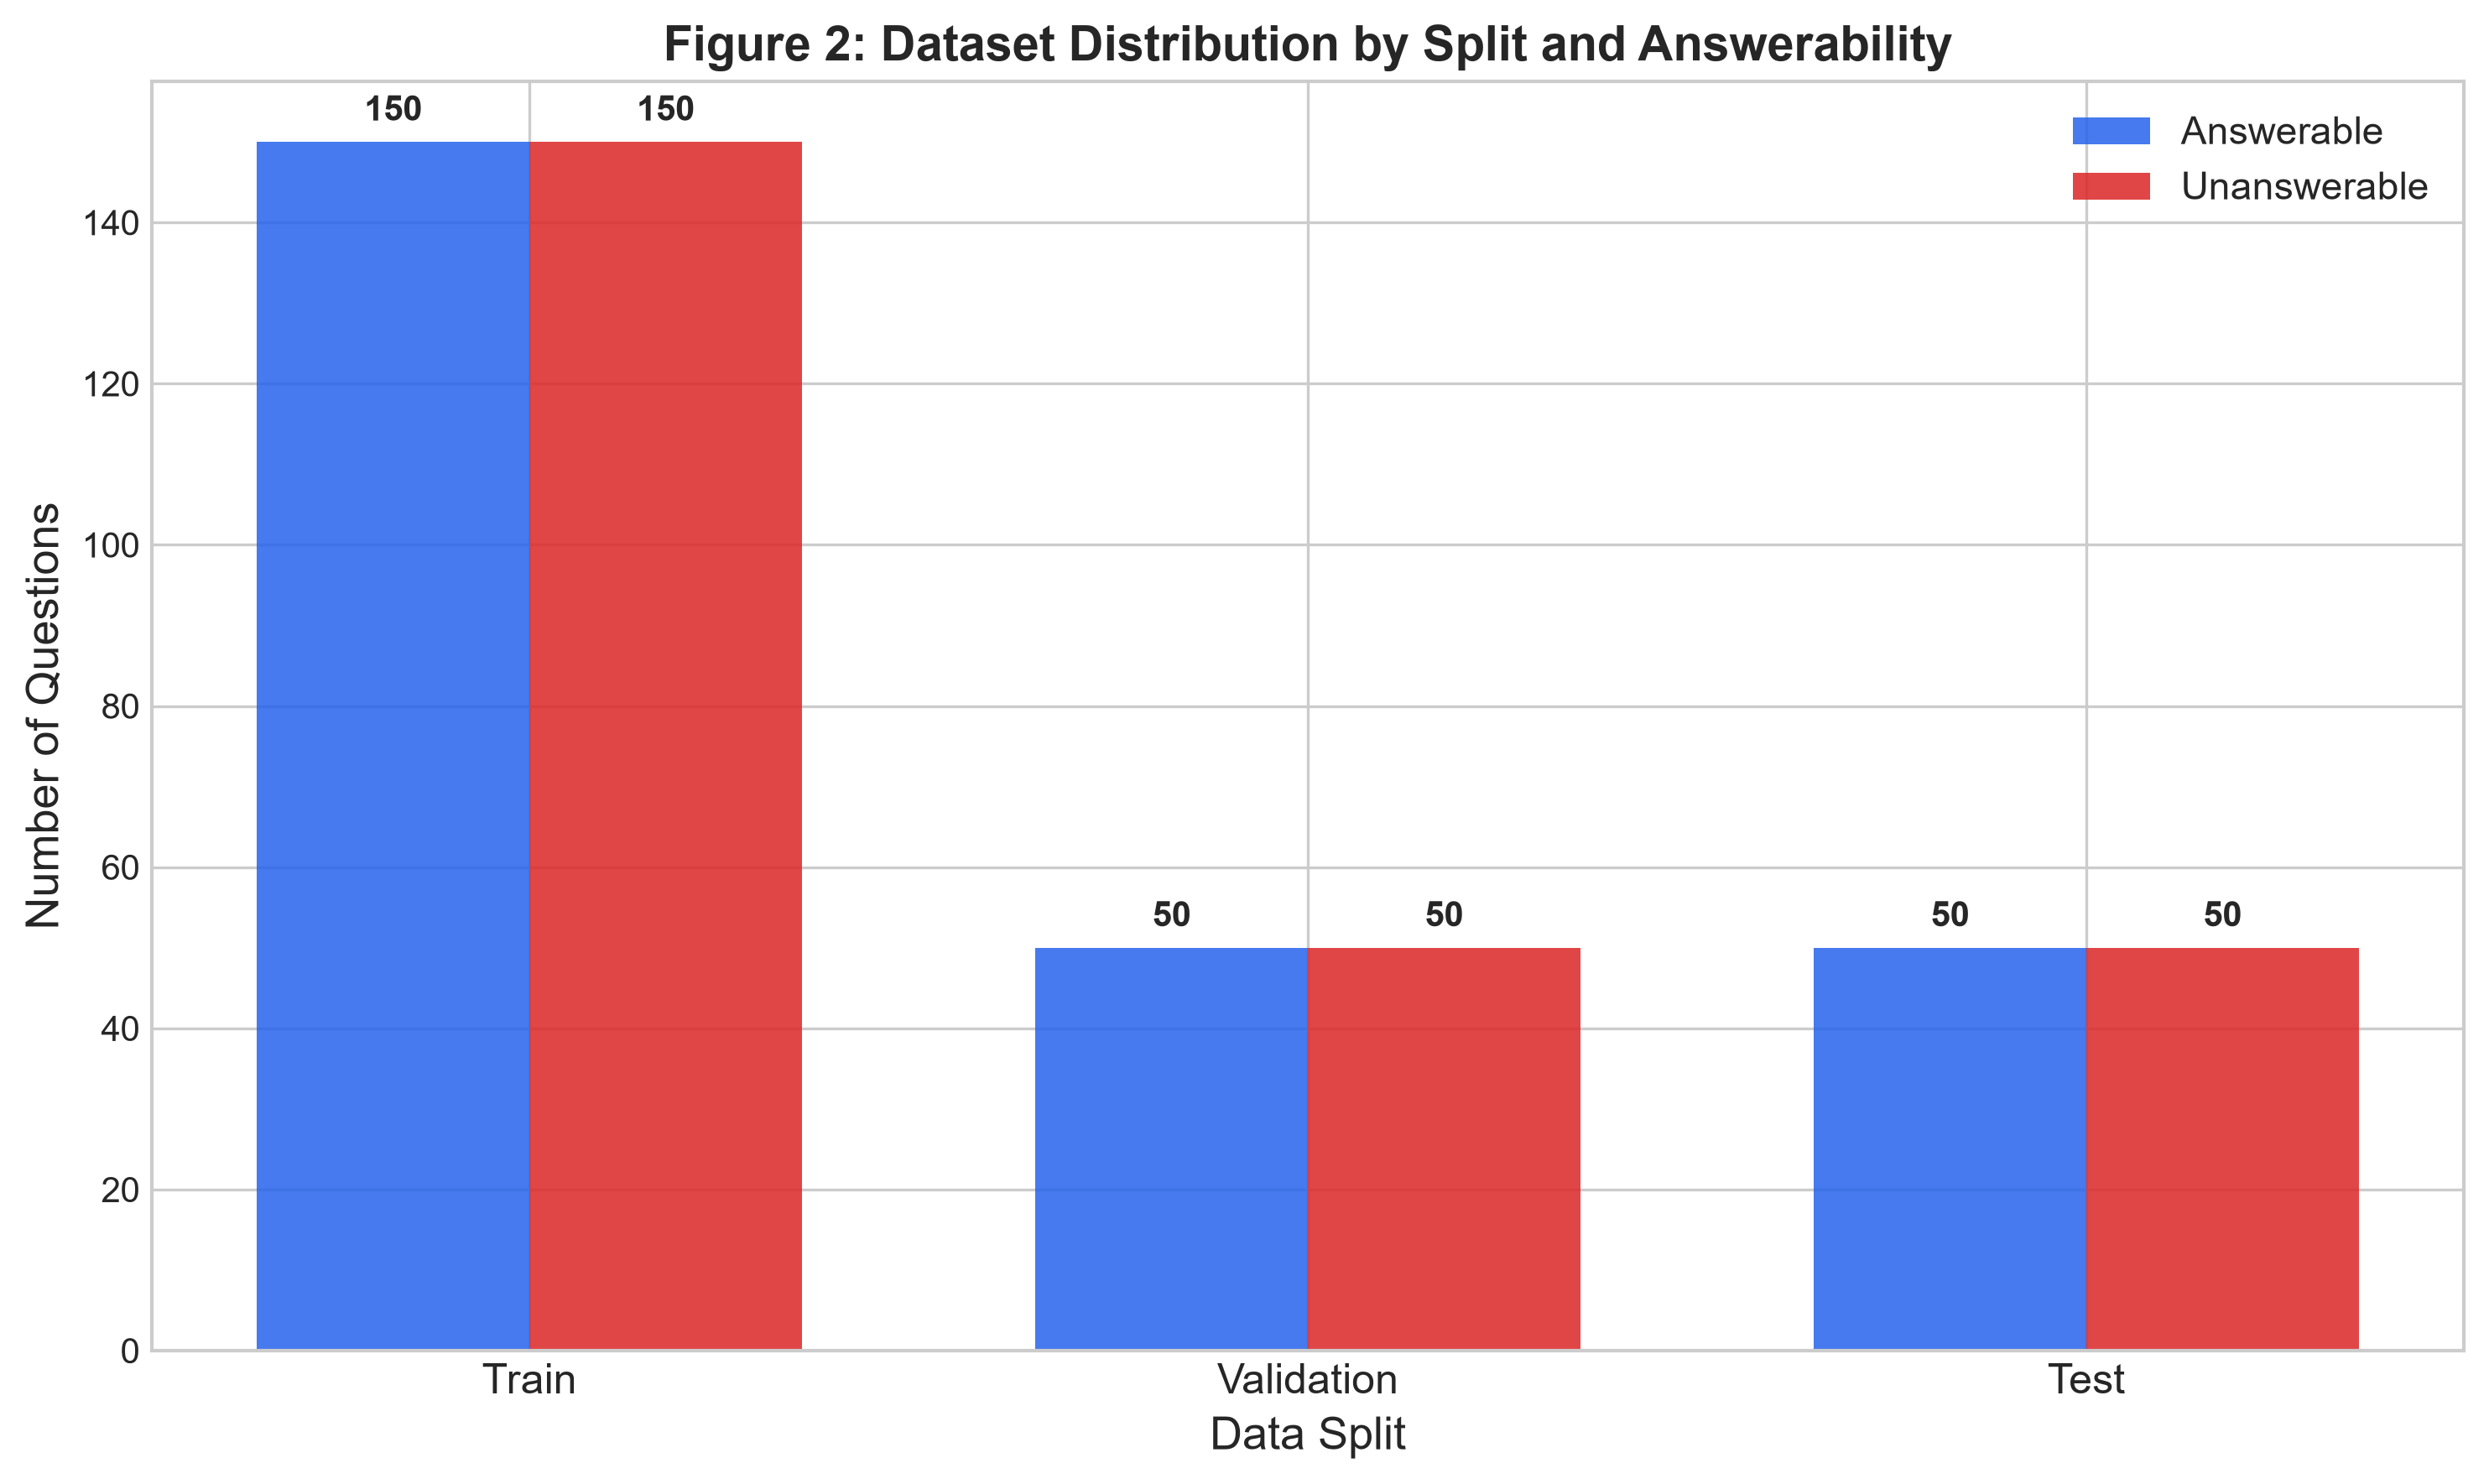
\includegraphics[width=0.80\textwidth]{fig2_dataset_distribution}
  \caption{Answerable vs.\ unanswerable question counts per data split.}
  \label{fig:dataset_distribution}
\end{figure}

\section{BM25 Configuration}
\label{sec:exp_bm25_config}

We use the \texttt{rank\_bm25} Python package (Okapi BM25 variant) with
default hyper-parameters: $k_1 = 1.5$, $b = 0.75$. Text is lower-cased and
split on whitespace before indexing. The top-$k = 5$ passages are retrieved
per query. Table~\ref{tab:bm25_stats} shows descriptive statistics for the
top-BM25-score feature across splits.

\begin{table}[htbp]
  \centering
  \caption{Descriptive statistics of \texttt{top\_bm25\_score} by data split.}
  \label{tab:bm25_stats}
  \begin{tabular}{lrrrr}
    \toprule
    \textbf{Split} & \textbf{Mean} & \textbf{Std} & \textbf{Min} & \textbf{Max} \\
    \midrule
    Train      & 30.89 & 13.13 &  4.49 & 107.21 \\
    Validation & 26.60 & 11.45 &  5.95 &  82.57 \\
    Test       & 26.69 & 12.02 &  4.98 & 112.81 \\
    \bottomrule
  \end{tabular}
\end{table}

Figures~\ref{fig:bm25_distribution} and \ref{fig:bm25_per_split} visualise the
BM25 score distributions by answerability label and by split, respectively.

\begin{figure}[htbp]
  \centering
  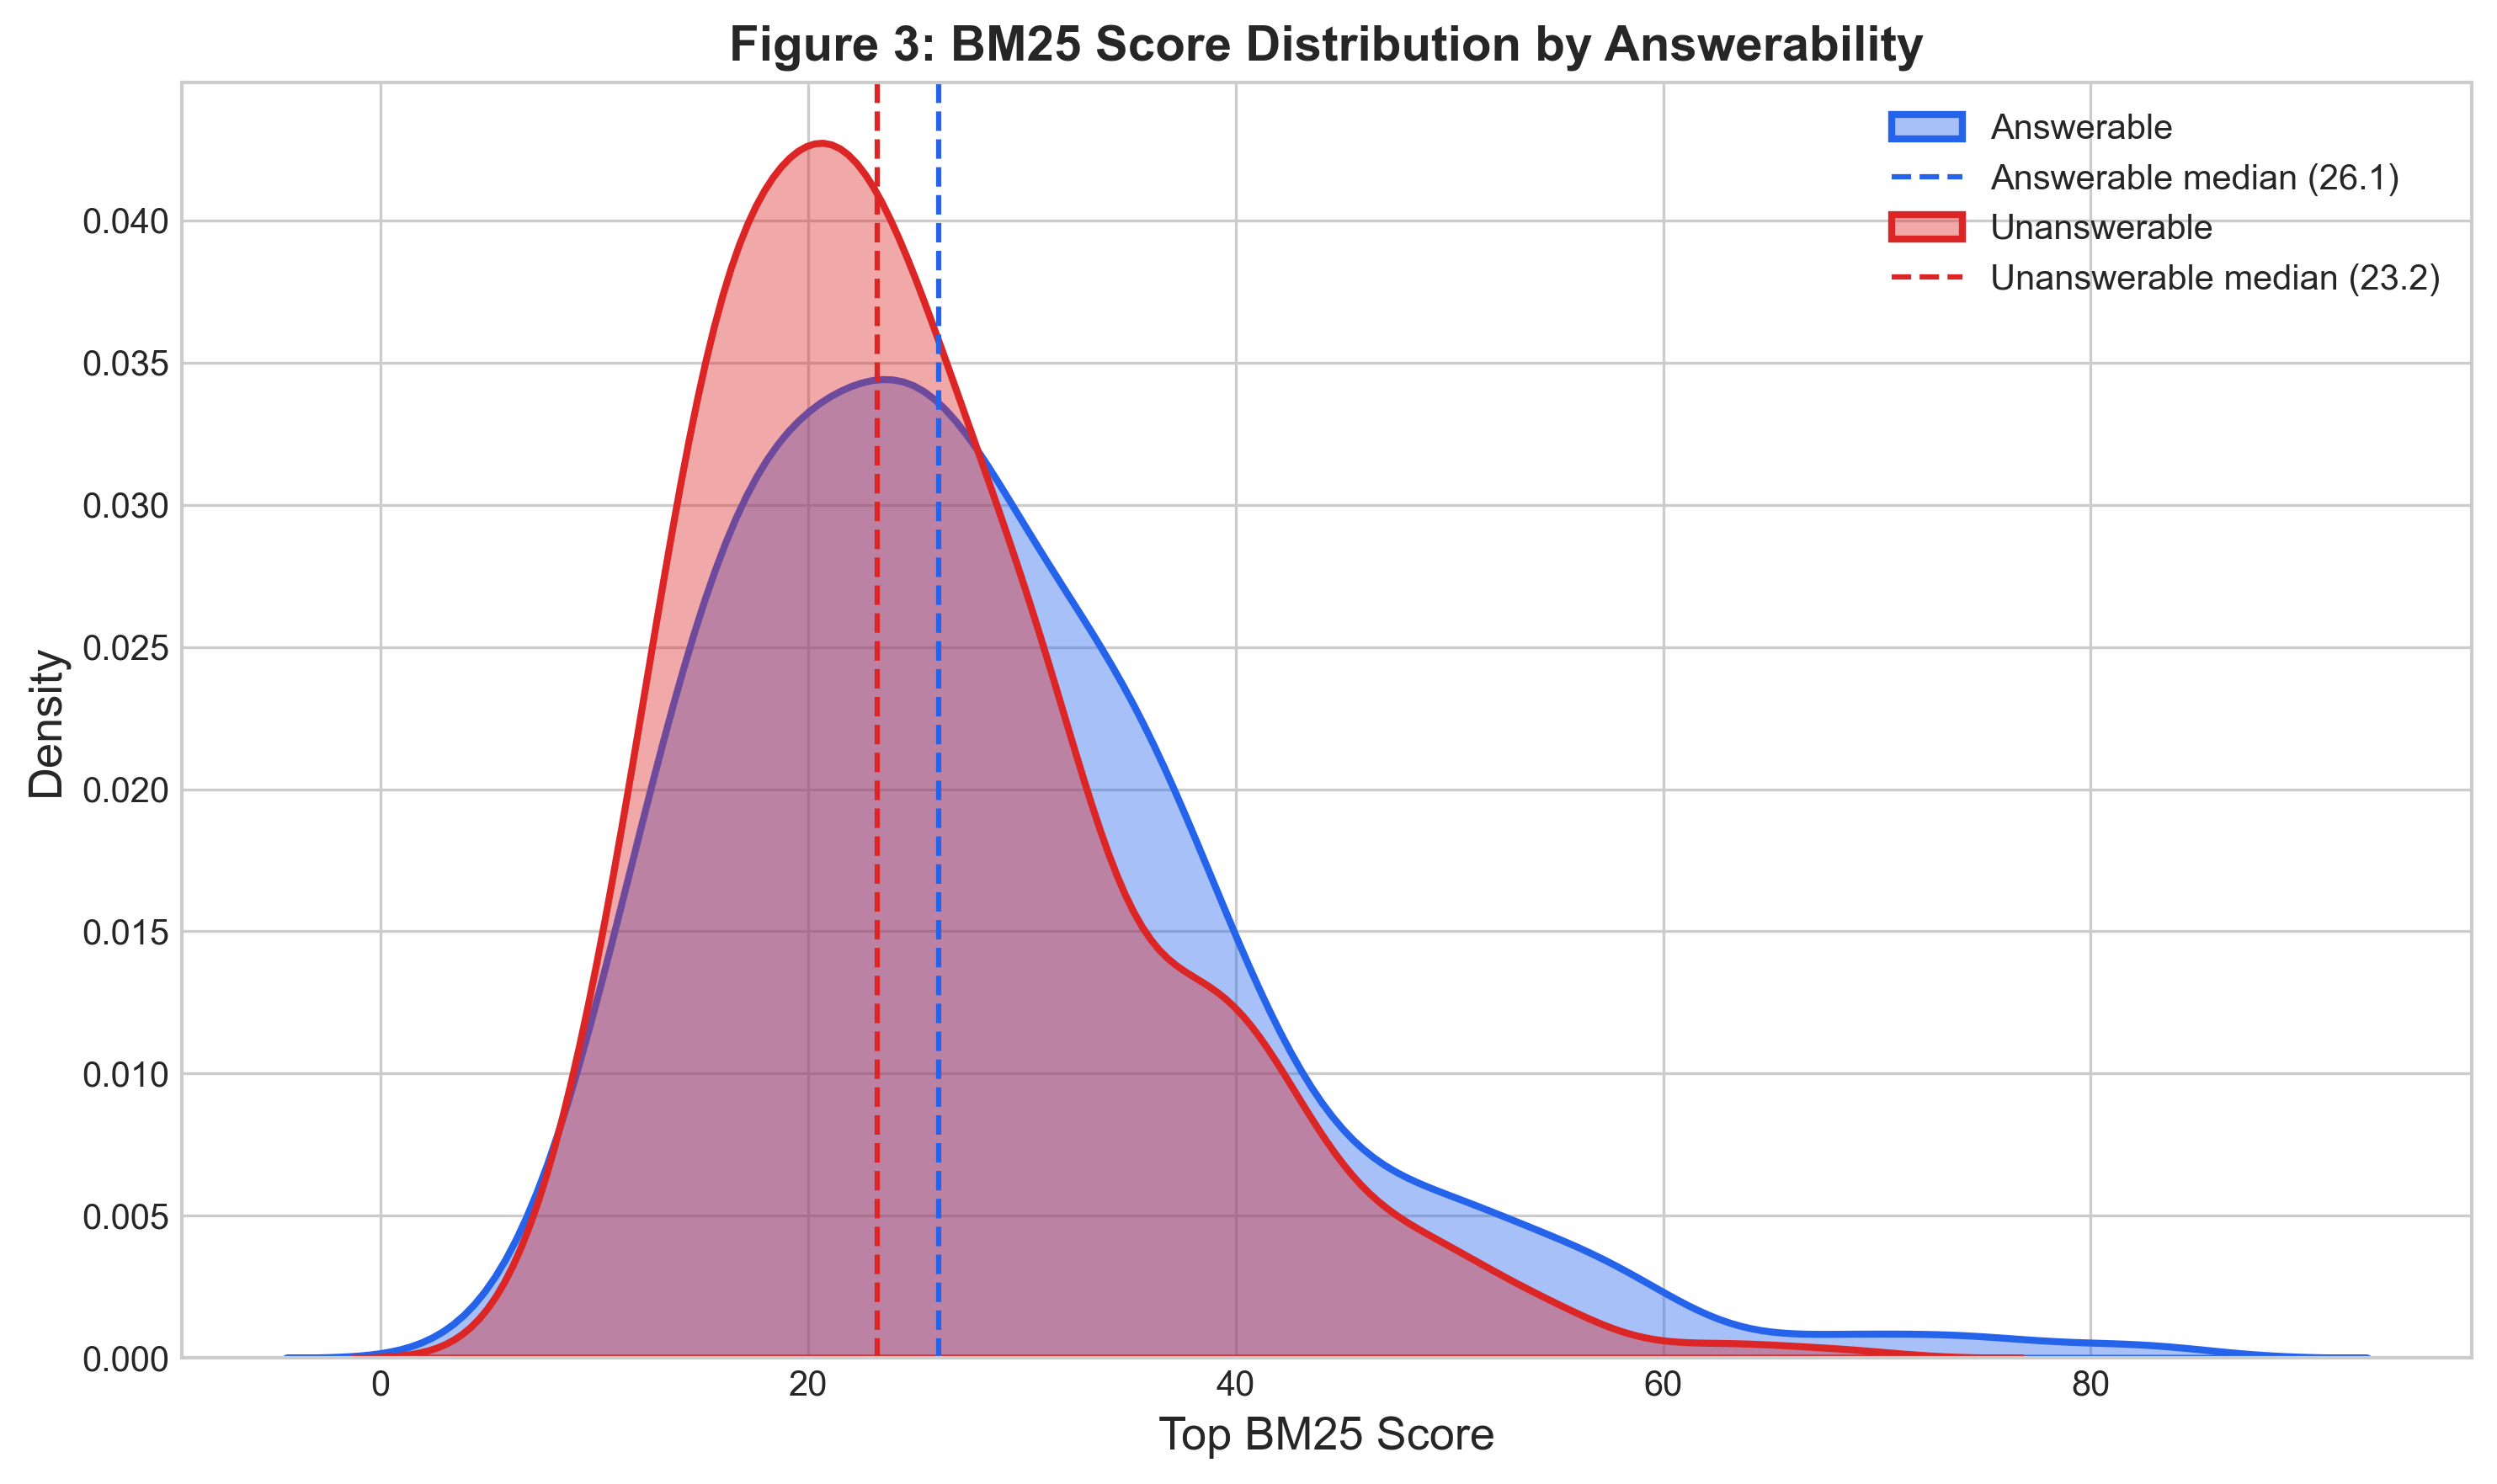
\includegraphics[width=0.80\textwidth]{fig3_bm25_score_distribution}
  \caption{Distribution of \texttt{top\_bm25\_score} for answerable vs.\
           unanswerable questions on the validation split.}
  \label{fig:bm25_distribution}
\end{figure}

\begin{figure}[htbp]
  \centering
  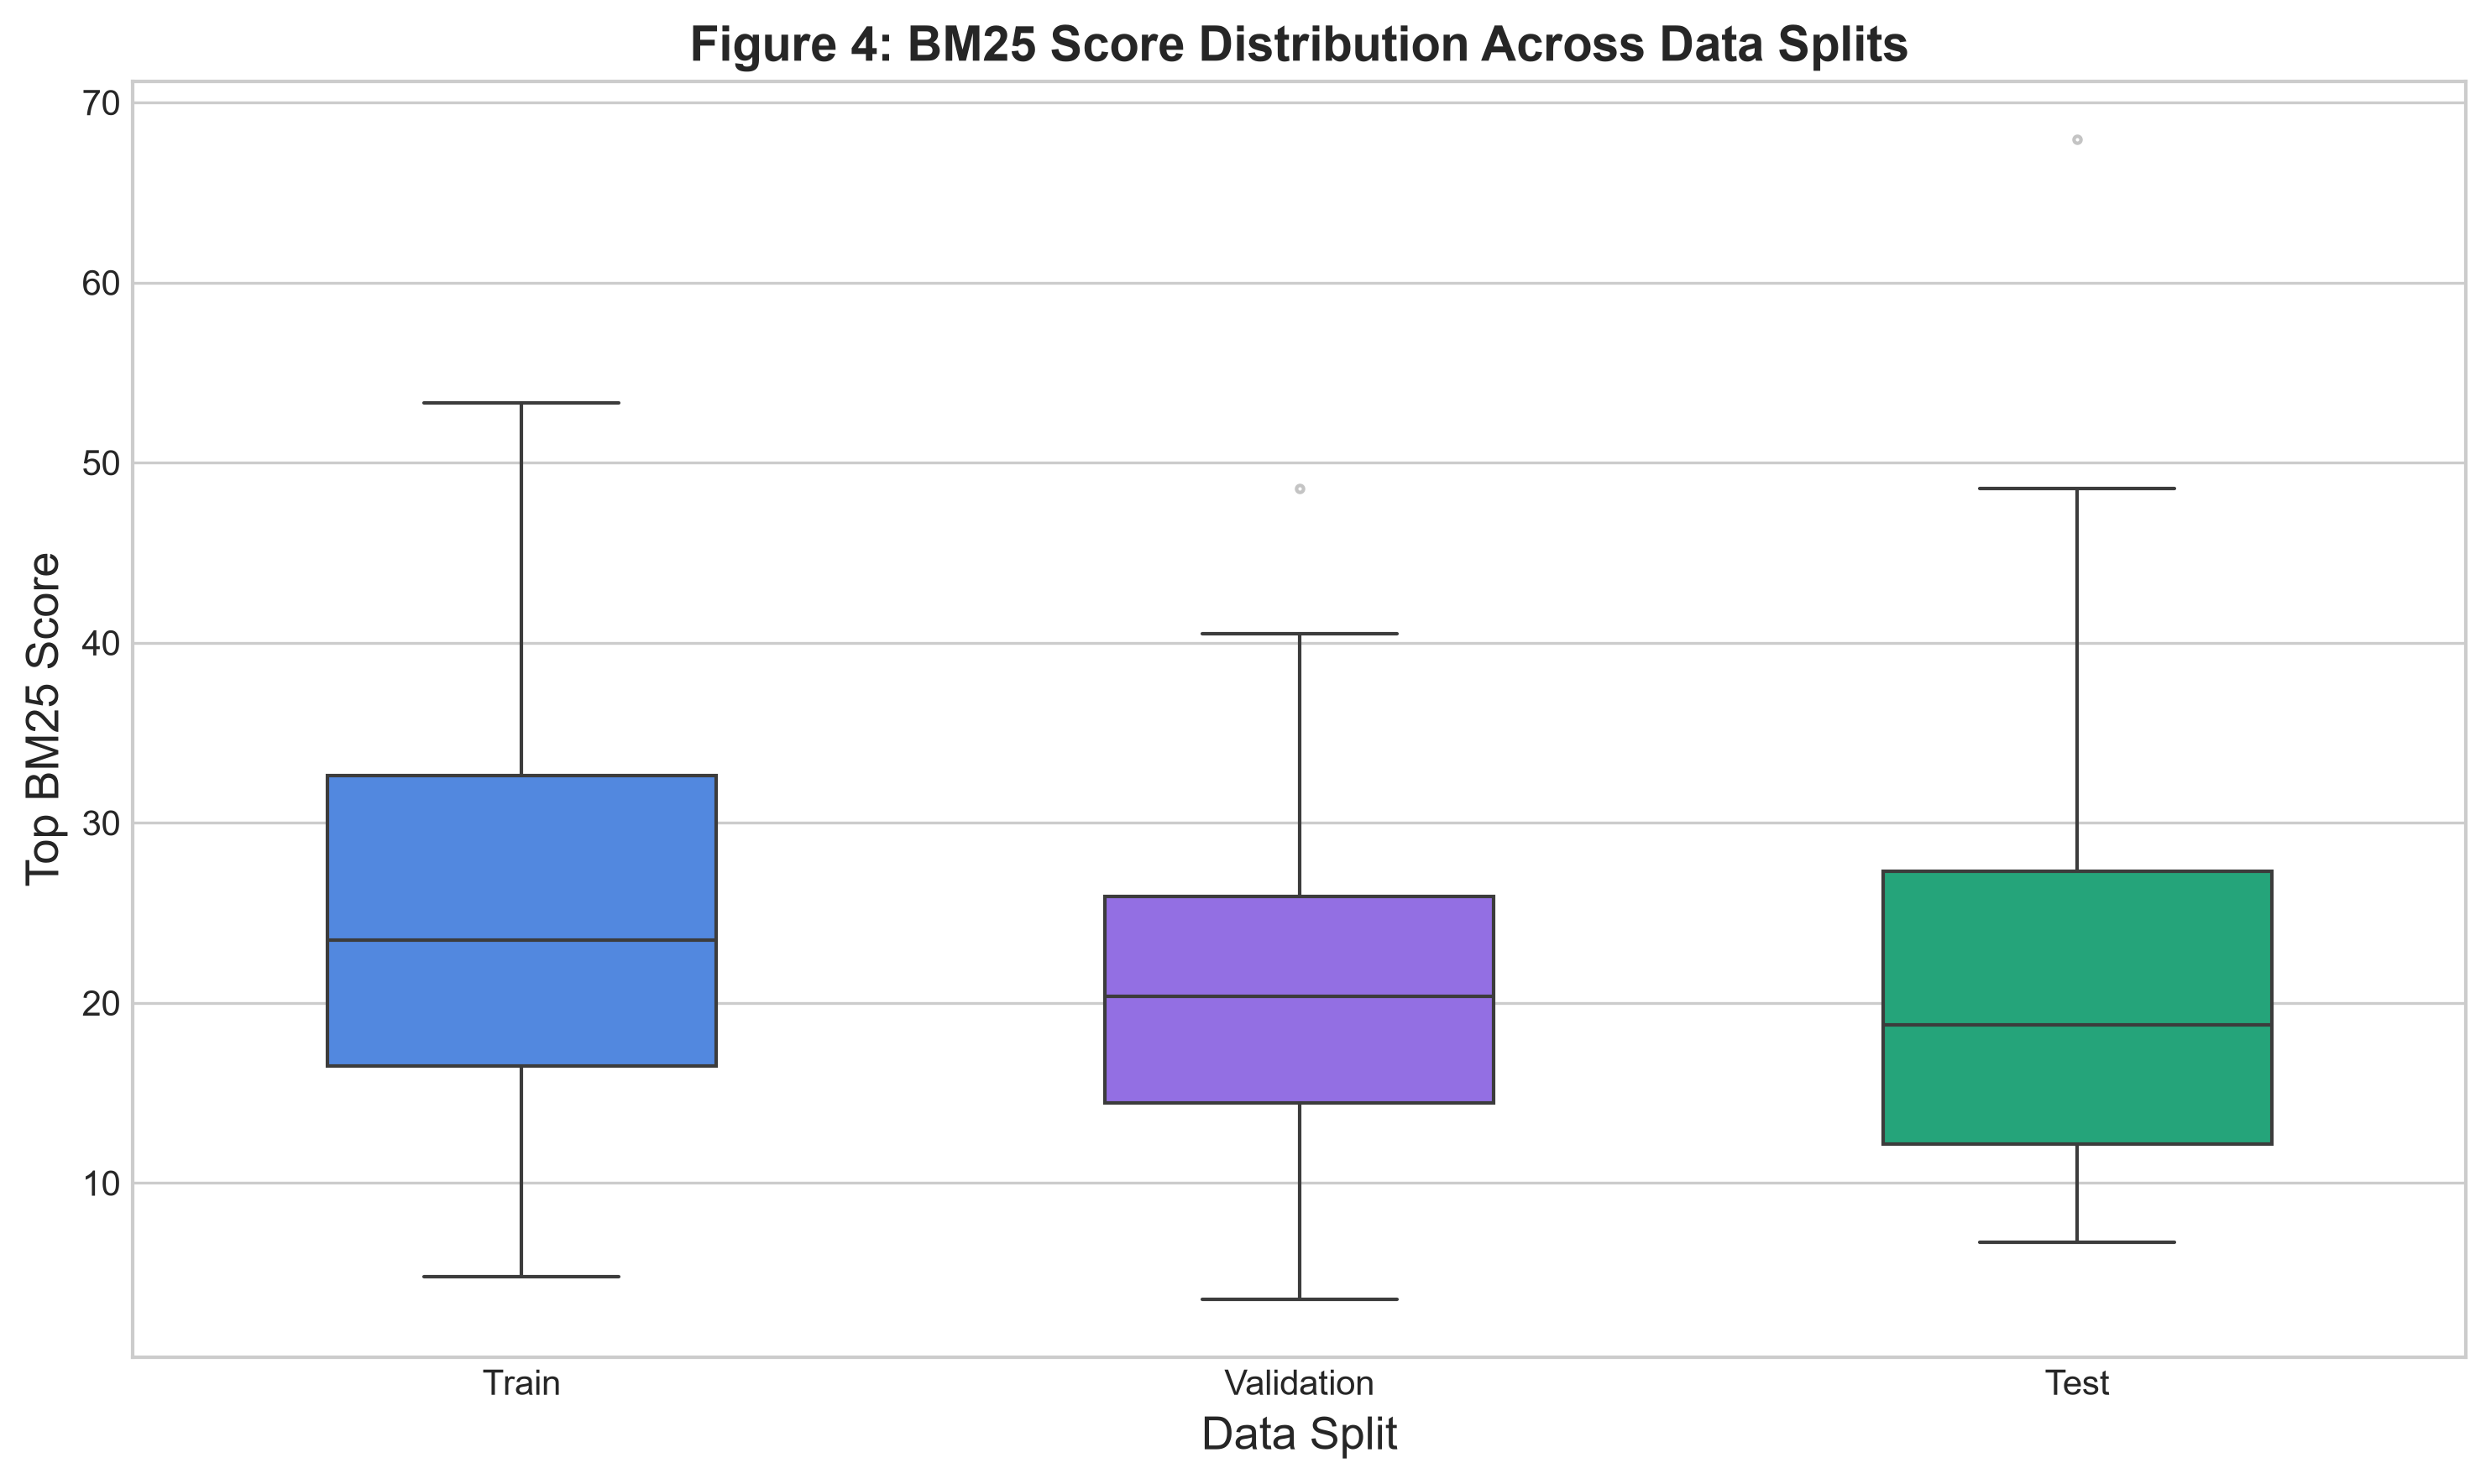
\includegraphics[width=0.80\textwidth]{fig4_bm25_scores_per_split}
  \caption{Box plots of \texttt{top\_bm25\_score} across data splits.}
  \label{fig:bm25_per_split}
\end{figure}

\section{QA Reader Configuration}
\label{sec:exp_reader_config}

\begin{itemize}
  \item \textbf{Model checkpoint:} \texttt{deepset/roberta-base-squad2} (Hugging
        Face Hub).
  \item \textbf{Task:} \texttt{question-answering} pipeline.
  \item \textbf{handle\_impossible\_answer:} \texttt{True}.
  \item \textbf{Passages per question:} 1 (top-1 BM25 result only).
  \item \textbf{Device:} CPU (or GPU if available; inference results are
        deterministic).
  \item \textbf{Max sequence length:} 512 tokens (model default).
\end{itemize}

On the test set, the \texttt{qa\_score} has mean $0.290$ ($\sigma = 0.365$),
ranging from near-zero to $0.996$, reflecting the range from clearly
unanswerable questions (low score) to highly confident extractable answers
(high score).

\section{Classifier Configuration}
\label{sec:exp_classifier_config}

\begin{itemize}
  \item \textbf{Model:} \texttt{LogisticRegression} (\texttt{sklearn}).
  \item \textbf{Solver:} LBFGS, maximum 2,000 iterations, balanced class weighting.
  \item \textbf{Regularisation:} L2, $C = 1.0$.
  \item \textbf{Pre-processing:} \texttt{SimpleImputer} (median strategy) $\rightarrow$
        \texttt{StandardScaler}.
  \item \textbf{Features:} 10 inference features (see Table~\ref{tab:features}).
  \item \textbf{Training data:} 300 training questions.
  \item \textbf{Threshold search:} $\delta \in [0.01, 0.99]$ step 0.01 on
        validation set (100 questions); best $\delta^* = 0.42$ ($\tau_{\text{BM25}} = 13.15$).
\end{itemize}

\section{Evaluation Protocol}
\label{sec:exp_eval_protocol}

For each question, the ground-truth label is \emph{answerable} (1) if
\texttt{is\_impossible}~$= 0$, else \emph{unanswerable} (0). An answer is
considered \emph{correct} if the system returns a non-empty string when the
question is answerable, or returns empty / abstains when the question is
unanswerable.

We compute the six metrics defined in Section~\ref{sec:meth_metrics}
(Precision, Recall, F1, Coverage, False-Answer Rate, False-Abstention Rate) on
the test set for each of the three strategies. The BM25 threshold and
classifier threshold are fixed to validation-tuned values before the test set
is evaluated. All computations are reproduced from the \texttt{results/}
directory using the saved prediction and decision CSV files.
